\documentclass[12pt]{article}

\usepackage{amsmath}
\usepackage{amsfonts}
\usepackage{listings}
\usepackage{float}
\usepackage{fancyhdr}
\usepackage{graphicx}
\usepackage[colorlinks=true,linkcolor=blue, citecolor=red]{hyperref}
\usepackage{url}
\usepackage[top=.75in, left=.5in, right=.5in, bottom=1in]{geometry}
\usepackage{parskip}
\usepackage[utf8]{vietnam}
\usepackage{xcolor}
\setlength{\headheight}{29.43912pt}

\definecolor{codegreen}{rgb}{0,0.6,0}
\definecolor{codegray}{rgb}{0.5,0.5,0.5}
\definecolor{codepurple}{rgb}{0.58,0,0.82}
\definecolor{backcolour}{rgb}{0.95,0.95,0.92}

\lstdefinestyle{mystyle}{
    backgroundcolor=\color{backcolour},   
    commentstyle=\color{codegreen},
    keywordstyle=\color{magenta},
    numberstyle=\tiny\color{codegray},
    stringstyle=\color{codepurple},
    basicstyle=\ttfamily\footnotesize,
    breakatwhitespace=false,         
    breaklines=true,                 
    captionpos=b,                    
    keepspaces=true,                 
    numbers=left,                    
    numbersep=5pt,                  
    showspaces=false,                
    showstringspaces=false,
    showtabs=false,                  
    tabsize=2
}

\lstset{style=mystyle}

% \graphicspath{PATH_TO_GRAPHIC_FOLDER}

\newcommand{\coursename}{CSC15008 - Xử lý ngôn ngữ tự nhiên ứng dụng}
\newcommand{\reportname}{Báo cáo Lab 04}

\pagestyle{fancy}
\lhead{
\reportname
}
\rhead{
Trường Đại học Khoa học Tự nhiên - ĐHQG HCM\\
\coursename
}
\lfoot{\LaTeX\ by \href{https://github.com/trhgquan}{Quan, Tran Hoang}}


\begin{document}

\begin{titlepage}
\newcommand{\HRule}{\rule{\linewidth}{0.5mm}}
\centering

\textsc{\LARGE đại học quốc gia tphcm}\\[1.5cm]
\textsc{\Large trường đại học khoa học tự nhiên}\\[0.5cm]
\textsc{\large khoa công nghệ thông tin}\\[0.5cm]
\textsc{bộ môn công nghệ tri thức}\\[0.5cm]

\HRule \\[0.4cm]
{ 
\huge{\bfseries{\reportname}}\\[0.5cm]
\large{\bfseries{Đề tài: Tìm hiểu phương pháp phân lớp văn bản khi các lớp được phân tầng}}
}\\[0.4cm]
\HRule \\[0.5cm]

\textbf{\large Môn học: \coursename}\\[0.5cm]

\begin{minipage}{0.4\textwidth}
\begin{flushleft} \large
\emph{Sinh viên thực hiện:}\\
Trần Hoàng Quân (19120338)
\end{flushleft}
\end{minipage}
~
\begin{minipage}{0.4\textwidth}
\begin{flushright} \large
\emph{Giáo viên hướng dẫn:} \\
Thầy Nguyễn Hồng Bửu Long
\end{flushright}
\end{minipage}\\[2cm]

{\large \today}\\[2cm]


\includegraphics[scale=.3]{img/hcmus-logo.png}\\[1cm] 

\vfill
\end{titlepage}

\tableofcontents
\listoffigures
\listoftables
\pagebreak

\section{Giới thiệu \& miêu tả bài toán}
Ngày nay nhiều phần mềm, ứng dụng tổ chức dữ liệu theo cấu trúc phân cấp, theo đó các lớp dữ liệu được chuyên biệt hóa thành những lớp con hoặc nhóm lại thành các lớp cha.\cite{huang2019hierarchical}

Hierarchical Multi-label Text Classification - \textbf{Phân lớp văn bản khi các lớp được phân tầng} là bài toán phân lớp văn bản mà mỗi lớp được tổ chức theo một cấu trúc phân cấp.

\textbf{Ví dụ:} xem hình sau.
\begin{figure}[H]
    \centering
    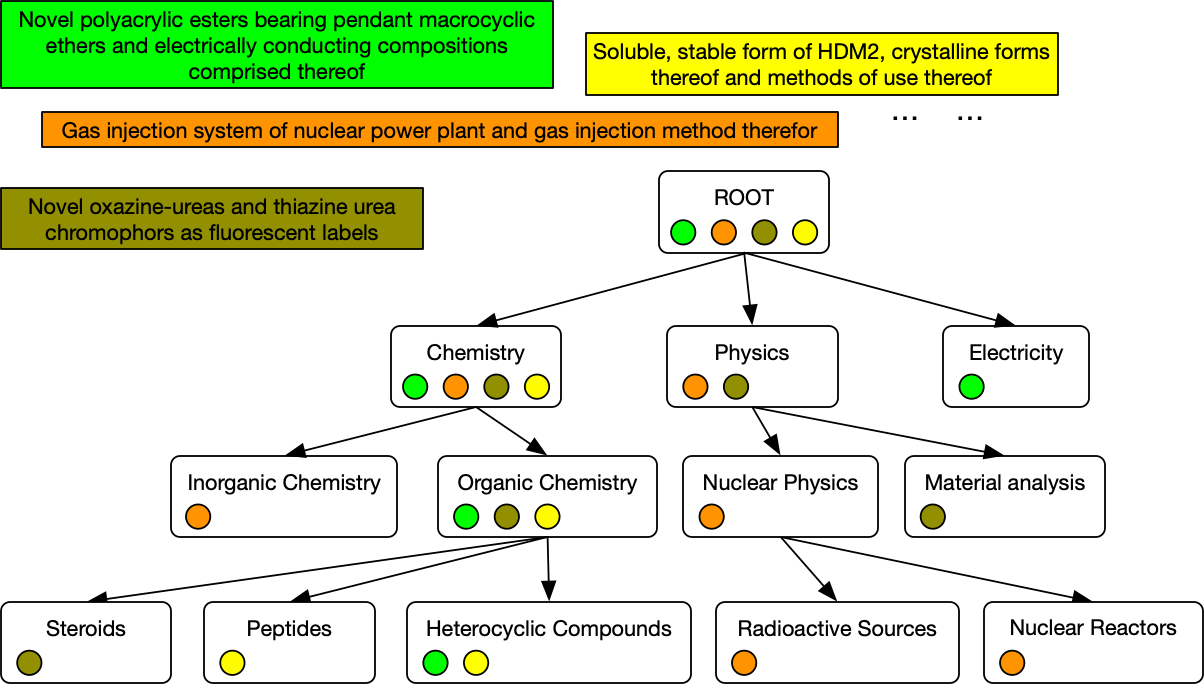
\includegraphics[scale=.5]{img/structure-demo.png}
    \caption{Ví dụ một trường hợp phân lớp phân tầng\cite{huang2019hierarchical}}
    \label{fig:example_hmtc}
\end{figure}
Ta cần phân lớp 4 đoạn văn vào các lớp:
\begin{itemize}
\item Chemistry (Hóa). Trong lớp này có 2 lớp con:
\begin{itemize}
    \item Inorganic Chemistry (Hóa vô cơ)
    \item Organic Chemistry (Hóa hữu cơ), gồm 3 lớp con:
    \begin{itemize}
        \item Steroids
        \item Peptides
        \item Heterocyclic Compounds
    \end{itemize}
\end{itemize}
\item Physics (Vật lí), trong lớp này có 2 lớp con:
\begin{itemize}
    \item Nuclear Physics (Vật lí hạt nhân), có 2 lớp con:
    \begin{itemize}
        \item Radioactive Sources
        \item Nuclear Reactors
    \end{itemize}
    \item Material Analysis
\end{itemize}
\item và Electricity (Điện)
\end{itemize}
Theo đó đoạn văn \textcolor{green}{màu xanh lá} được xếp vào lớp Chemistry và Electricity. Trong lớp Chemistry, đoạn văn được xếp vào lớp con Organic Chemistry. Trong lớp Organic Chemistry, đoạn văn thuộc lớp con Heterocyclic Compounds.

Công cụ được sử dụng trong báo cáo này sử dụng mạng neural hồi quy (RNN) theo cơ chế Attention. Kiến trúc mạng neural sử dụng trong paper gốc như sau:
\begin{figure}[H]
    \centering
    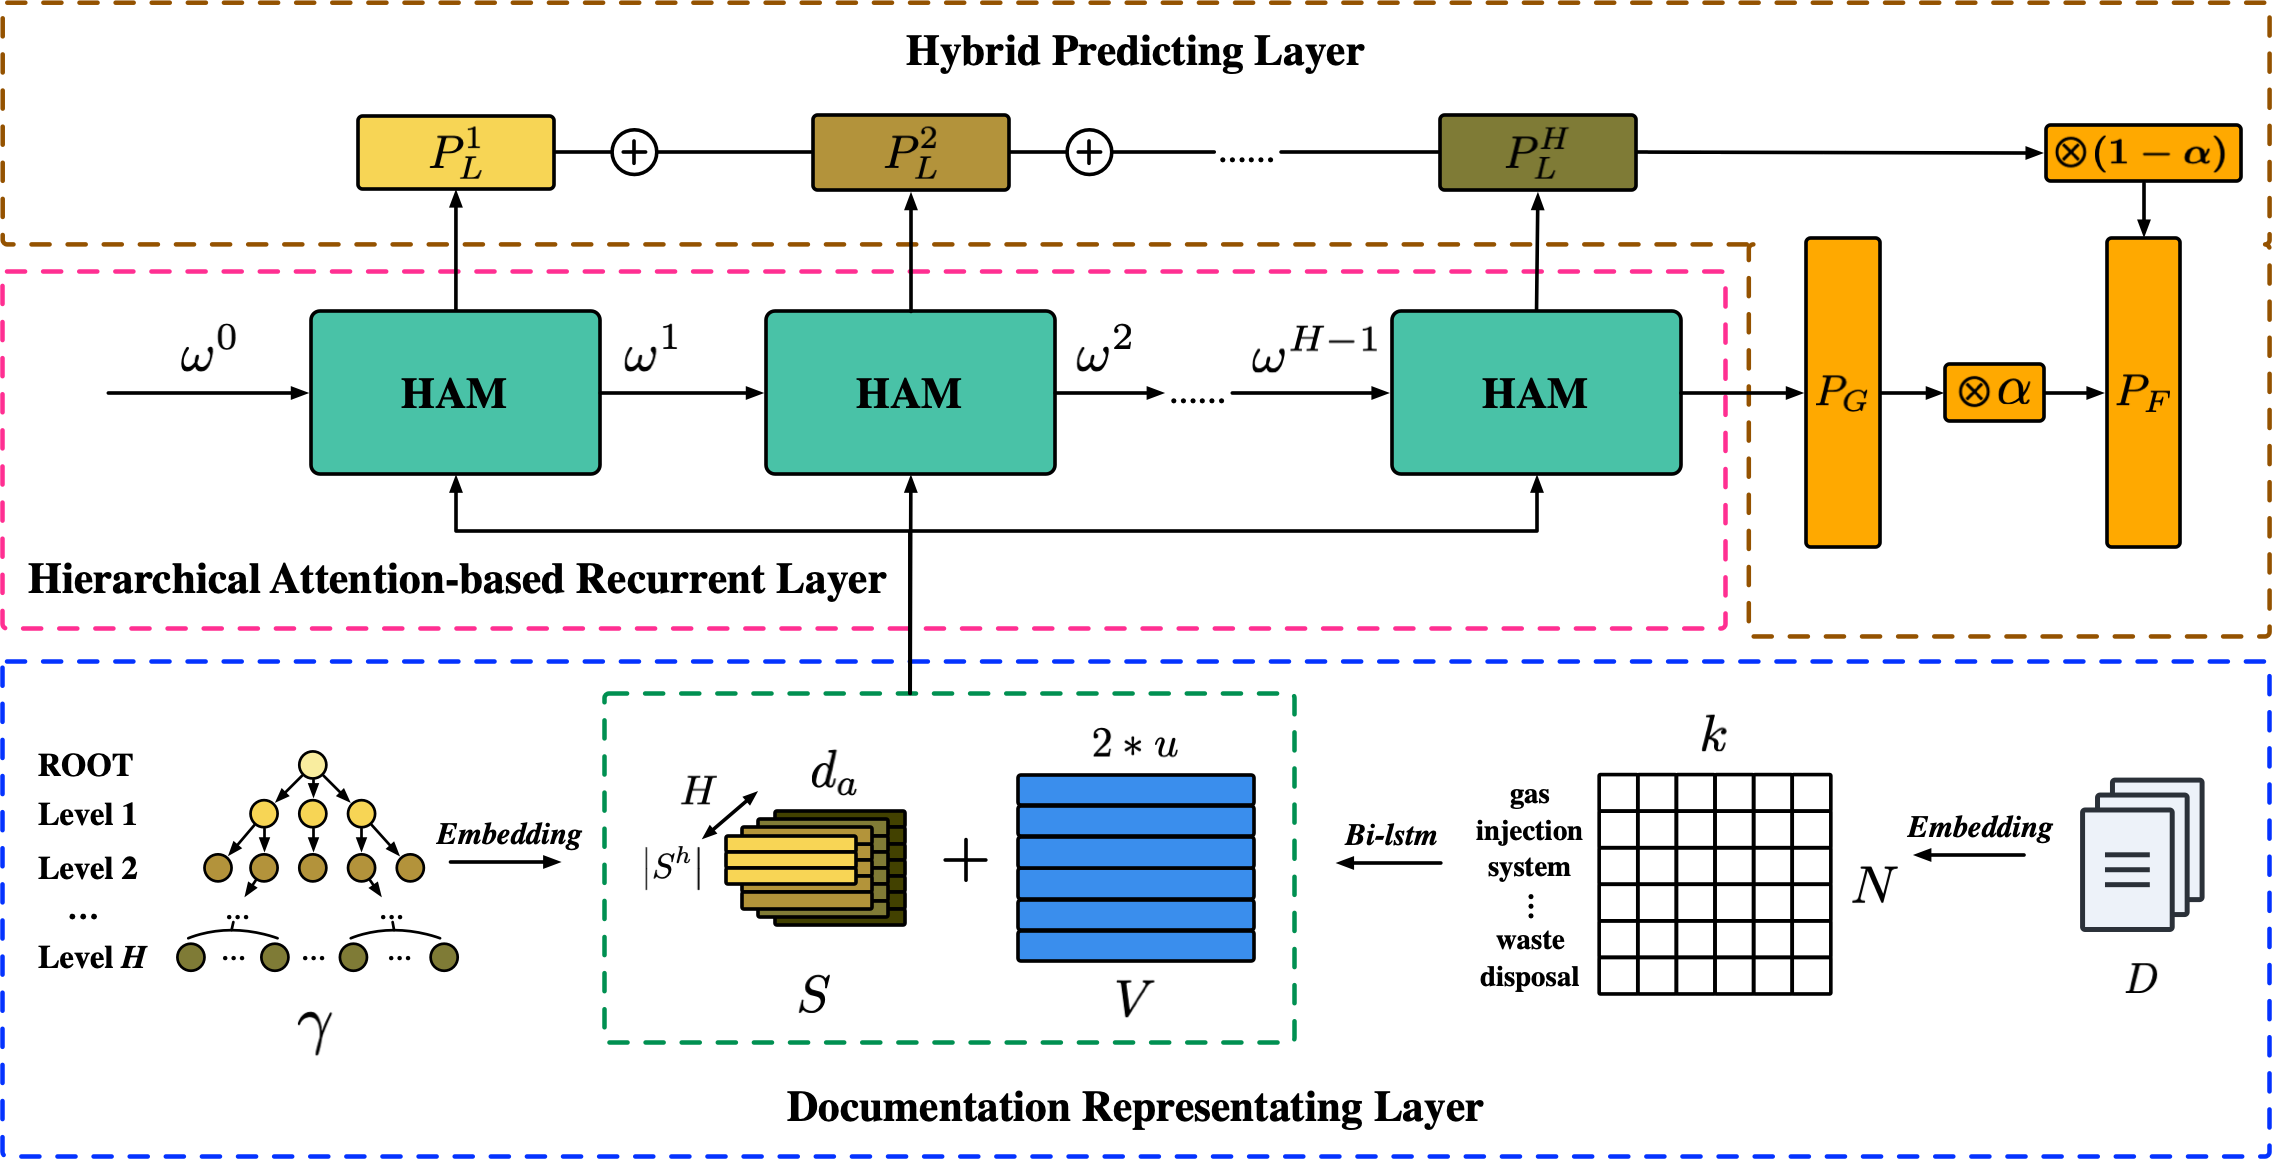
\includegraphics[scale=.25]{img/neural-structure.png}
    \caption{Kiến trúc mạng neural sử dụng trong bài báo\cite{huang2019hierarchical}}
    \label{fig:neural_structure}
\end{figure}

Đường link đến công cụ ở đây: \href{https://github.com/RandolphVI/Hierarchical-Multi-Label-Text-Classification}{RandolphVI/Hierarchical-Multi-Label-Text-Classification}

\section{Các câu lệnh cần sử dụng}
\subsection{Cài đặt package}
Ta cần cài đặt các package cần thiết\ref{notice}, sử dụng \texttt{pip}:
\begin{lstlisting}
pip install -r requirements.txt
\end{lstlisting}

\subsection{Data format}
Đảm bảo data đã được format thành file \texttt{.json} như ví dụ trên GitHub và đặt trong thư mục \texttt{data}. Ta cũng đảm bảo file word2vec đã được download và giải nén trong thư muc \texttt{data}.
\begin{itemize}
    \item Text segmentation: dùng \texttt{nltk}.
    \item Word2Vec: có thể sử dụng package \texttt{gensim} hoặc \texttt{glove}.
\end{itemize}

Link download data mẫu và cách format data, xin tham khảo GitHub của công cụ.

\subsection{Huấn luyện}
\begin{enumerate}
    \item Tiến hành huấn luyện model bằng cách chạy \texttt{HARNN/train\_harnn.py}:
    \begin{lstlisting}
    python train_harnn.py --train-file=<training file>.json --validation-file=<validation file>.json --test-file=<testing file>.json --epochs=<number of epochs> --batch-size=<batch size> --learning-rate=<adam learning rate>
    \end{lstlisting}
    \item Nhấn \textbf{T} để huấn luyện, \textbf{R} để quay lại huấn luyện nếu việc huấn luyện đã được tạm dừng ví lí do nào đó.
\end{enumerate}

\subsection{Test}
Thực hiện các bước như sau:
\begin{enumerate}
    \item Chạy \texttt{HARNN/test\_harnn.py} để tiến hành test.
    \begin{lstlisting}
    python test_harnn.py
    \end{lstlisting}
    \item Nhập file model muốn test (thường là 10 chữ số)
    \item Chọn model tốt nhất (best model - nhấn \textbf{B}) hoặc model mới nhất vừa train (latest model - nhấn \textbf{L})
\end{enumerate}
File \texttt{predictions.json} nằm trong thư mục \texttt{output/<id file model>} lưu kết quả prediction.

\section{Demo}
\subsection{Chạy thử}
Ngữ liệu được sử dụng là ngữ liệu mặc định trong folder \texttt{data}. Tiến hành train với \texttt{epochs = 10, batch size = 64}:
\begin{figure}[H]
    \centering
    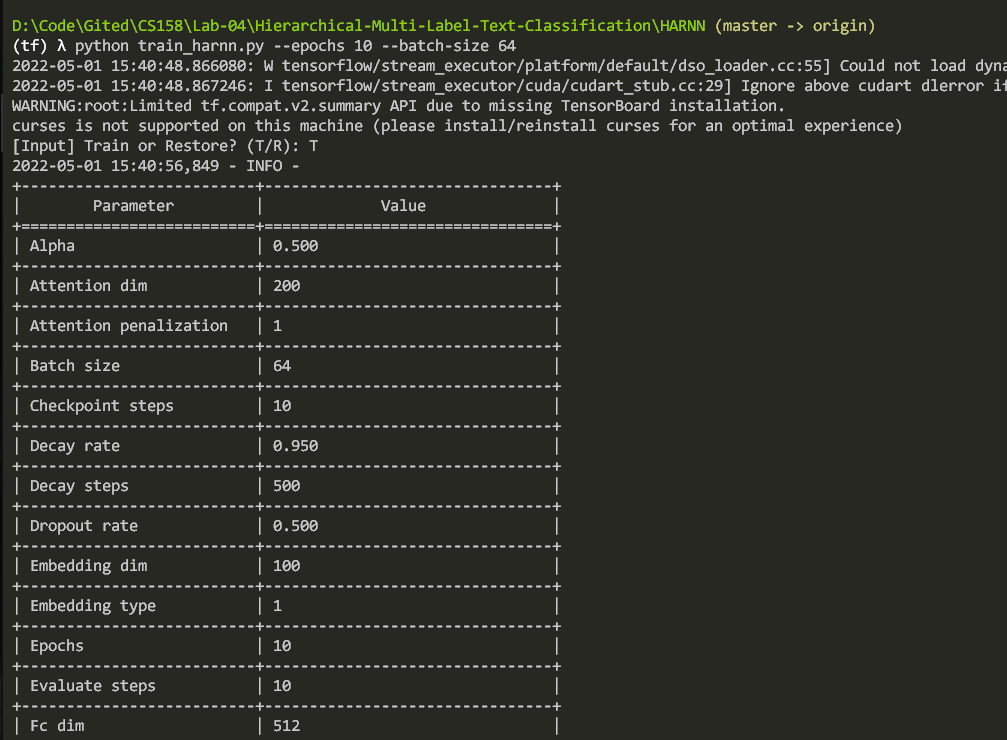
\includegraphics[scale=.5]{img/start-training.PNG}
    \caption{Bắt đầu train}
    \label{fig:start_training}
\end{figure}

Kích thước folder result khá lớn, dù input chỉ có 118KB:
\begin{figure}[H]
    \centering
    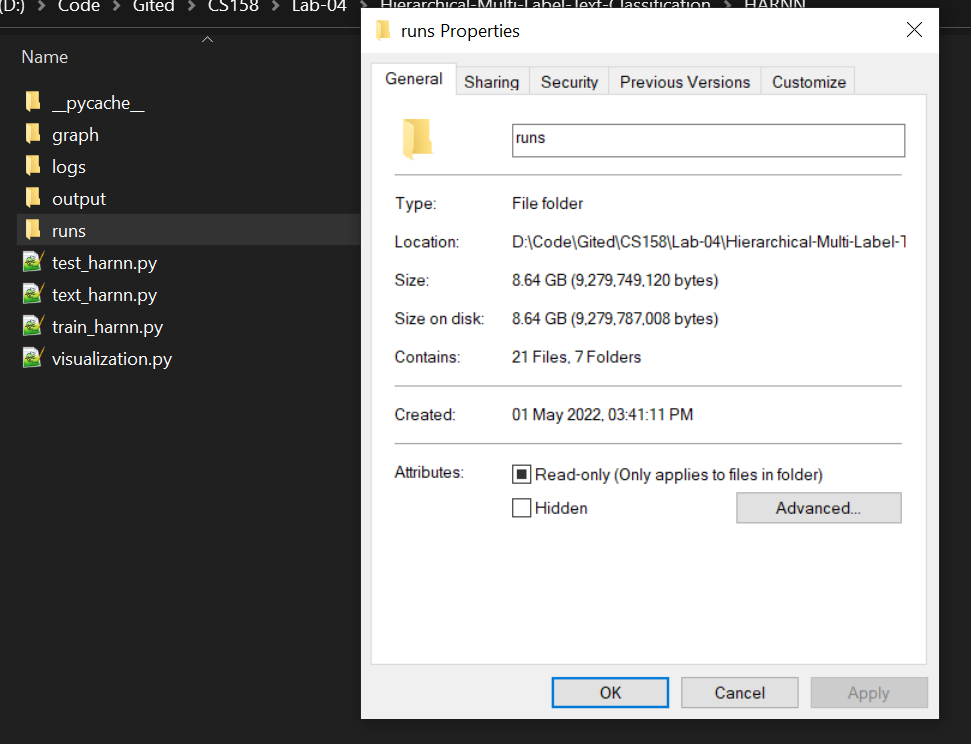
\includegraphics[scale=.7]{img/output-size.PNG}
    \caption{Kích thước folder output}
    \label{fig:output_size}
\end{figure}

Tiến hành test:
\begin{figure}[H]
    \centering
    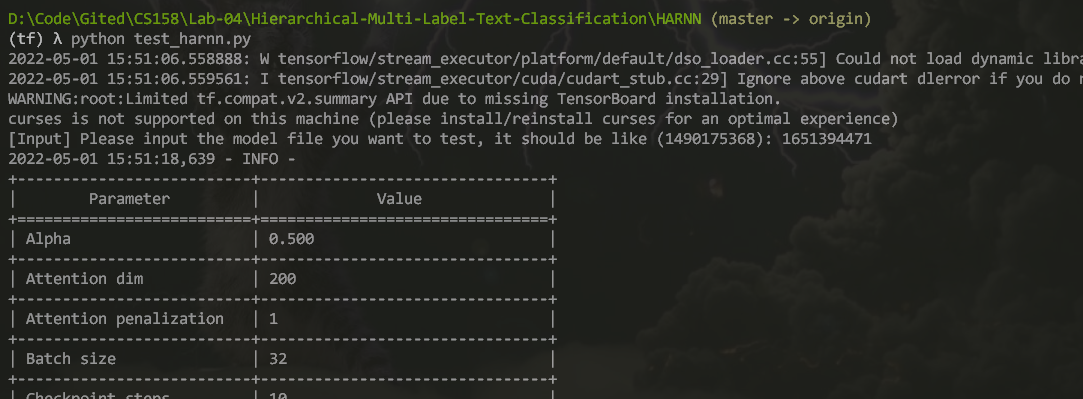
\includegraphics[scale=.7]{img/start-testing.PNG}
    \caption{Câu lệnh test}
    \label{fig:start_testing}
\end{figure}

Và kết quả test (sử dụng model tốt nhất):
\begin{figure}[H]
    \centering
    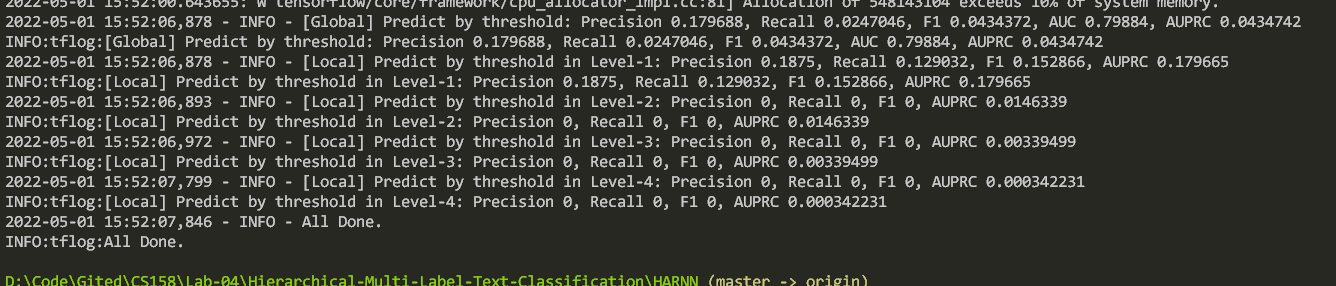
\includegraphics[scale=.65]{img/test-result.PNG}
    \caption{Kết quả test}
    \label{fig:testing_result}
\end{figure}
\begin{table}[H]
    \centering
    \begin{tabular}{|c|c|c|c|c|}
        \hline
        & Precision & Recall & F1 & AUPRC \\
        \hline
        Level-1 & 0.1875 & 0.129032 & 0.152866 & 0.179665 \\
        Level-2 & 0 & 0 & 0 & 0.0146339 \\
        Level-3 & 0 & 0 & 0 & 0.00339499 \\
        Level-4 & 0 & 0 & 0 & 0.000342231 \\
        \hline
    \end{tabular}
    \caption{Kết quả test}
    \label{tab:my_label}
\end{table}
File \texttt{predictions.json} có nội dung như sau:
\begin{figure}[H]
    \centering
    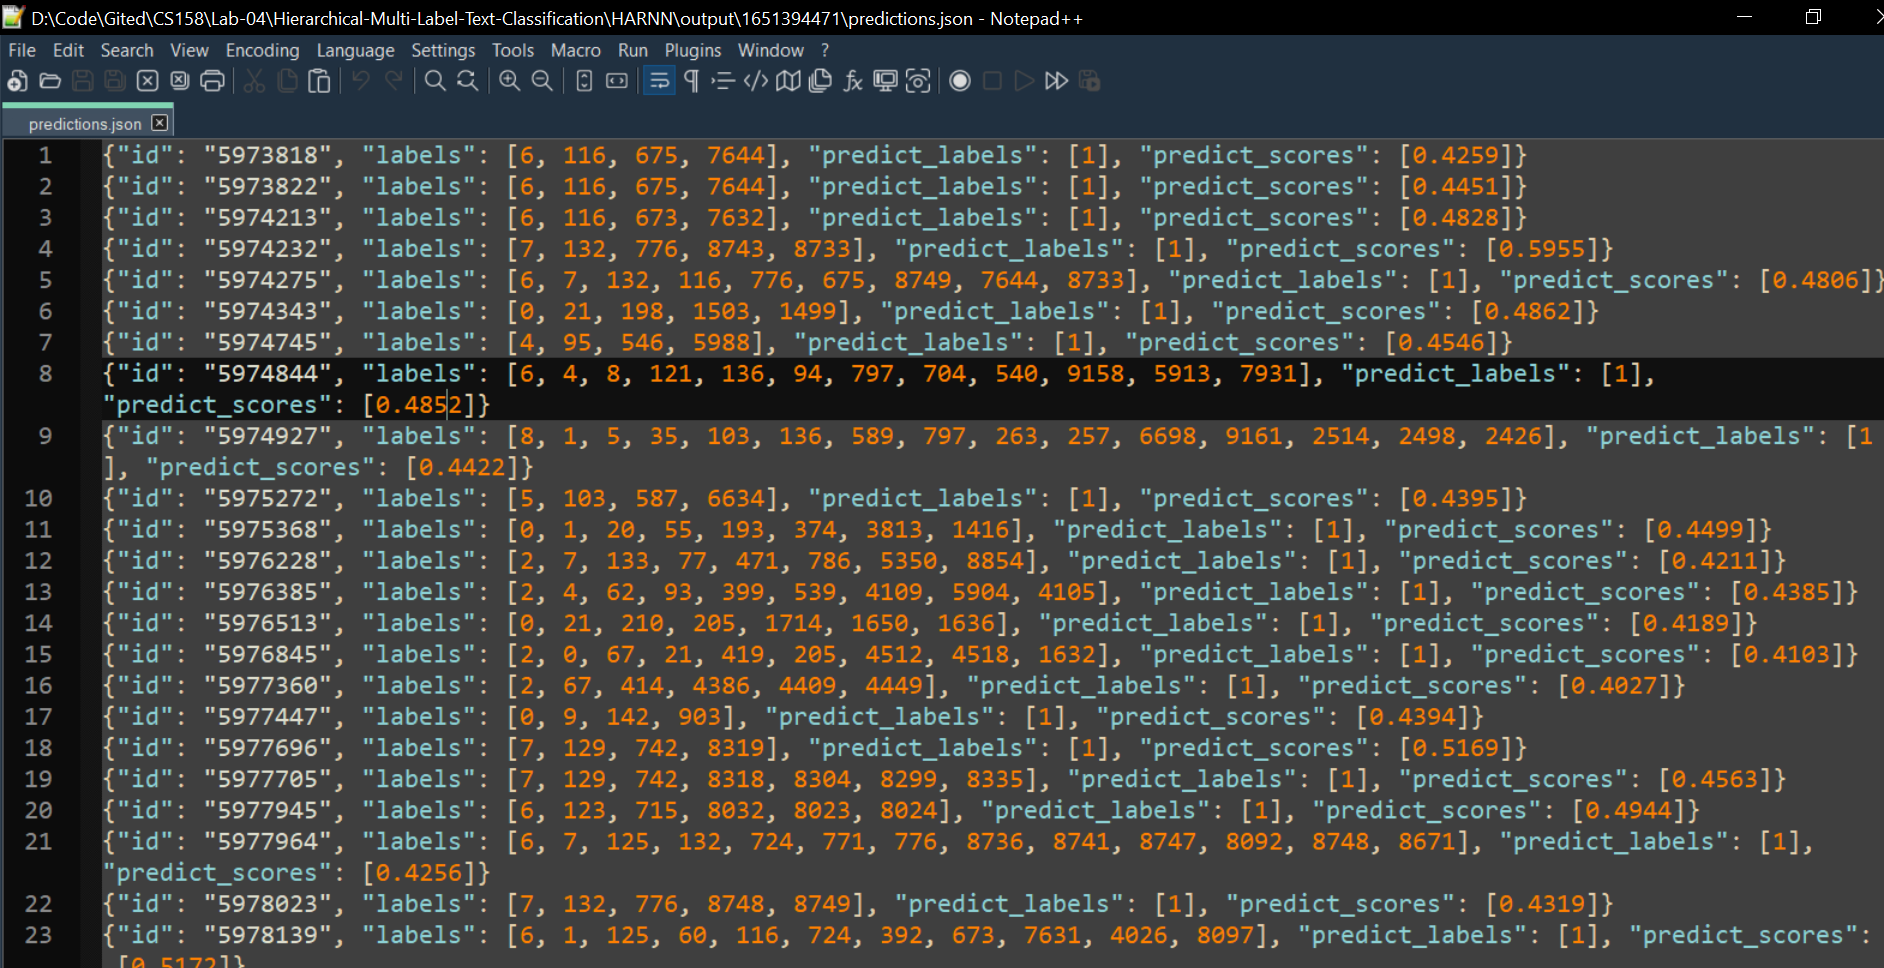
\includegraphics[scale=.45]{img/predictions-json.PNG}
    \caption{Nội dung \texttt{predictions.json}}
    \label{fig:predictions_json}
\end{figure}

\subsection{Nhận xét}
Vì kích thước dữ liệu sau khi huấn luyện quá lớn và thời gian huấn luyện quá lâu, nên trong bài báo cáo không sử dụng ngữ liệu được tác giả giới thiệu (Patient Dataset / Education Dataset).

Tuy nhiên, bước đầu huấn luyện và test cho ra kết quả khá chính xác, precision = 0.17 chỉ với 10 epochs và mỗi batch có kích thước 64. Nếu tăng số lượng epochs và batch size lên thì có thể dễ dàng đạt được độ chính xác cao hơn.

Một số lưu ý khi sử dụng công cụ:
\begin{itemize}
    \item Nên kích hoạt \texttt{venv} của anaconda và cài Python 3.6, một số package của công cụ đã outdated từ rất lâu và khó cài được bằng \texttt{pip install} thông thường.\label{notice}
    \item Cần cấu hình máy tương đối mạnh để huấn luyện, có thể cần thêm GPU mạnh.
    \item Trên môi trường Windows dễ gặp phải Python Error22. Đây là lỗi do cú pháp đặt tên file logs có dấu \texttt{:} là dấu không hợp lệ với tên file trên Windows. Thay dấu \texttt{:} ở dòng code đặt tên file logs đi là ổn.
\end{itemize}

\cleardoublepage
\phantomsection

\addcontentsline{toc}{section}{Tài liệu}
\bibliographystyle{plain}
\bibliography{sample}

\end{document}